\documentclass[11pt,letterpaper]{report}
\usepackage[utf8]{inputenc}
\usepackage[left=1in,right=1in,top=1in,bottom=1in]{geometry}
\usepackage{amsfonts,amsmath}
\usepackage{graphicx,float}
\usepackage{titlesec}
% -----------------------------------
\usepackage{hyperref}
\hypersetup{%
  colorlinks=true,
  linkcolor=blue,
  citecolor=blue,
  urlcolor=blue,
  linkbordercolor={0 0 1}
}
% -----------------------------------
\setlength{\parindent}{0.0in}
\setlength{\parskip}{0.1in}
% -----------------------------------
\newcommand{\de}{\mathrm{d}}
\newcommand{\DD}{\mathrm{D}}
\newcommand{\pe}{\partial}
\newcommand{\mcal}{\mathcal}
%\newcommand{\pdx}{\left|\frac{\partial}{\partial_x}\right|}

\newcommand{\dsp}{\displaystyle}

\newcommand{\norm}[1]{\left\Vert #1 \right\Vert}
%\newcommand{\mean}[1]{\left\langle #1 \right\rangle}
\newcommand{\mean}[1]{\overline{#1}}
\newcommand{\inner}[2]{\left\langle #1,#2\right\rangle}

\newcommand{\ve}[1]{\boldsymbol{#1}}

\newcommand{\thus}{\Rightarrow \quad }
\newcommand{\fff}{\iff\quad}
\newcommand{\qdt}[1]{\quad \mbox{#1} \quad}

\renewcommand{\Re}{\mathrm{Re}}
\renewcommand{\Im}{\mathrm{Im}}
\newcommand{\E}{\mathbb{E}}
\newcommand{\lap} {\nabla^2}
\renewcommand{\div}{\nabla\cdot}

\newcommand{\csch}{\text{csch}}
\newcommand{\sech}{\text{sech}}


\newcommand{\hot}{\text{h.o.t.}}

\newcommand{\ssp}{\left.\qquad\right.}

\newcommand{\var}{\text{var}}
\newcommand{\cov}{\text{cov}}

%%%%%%%%%%%%%%%%%%%%%%%%%%%%%%%%%%%%%%%%%%%%%%%%%%
\makeatletter
\newcommand*{\mint}[1]{%
  % #1: overlay symbol
  \mint@l{#1}{}%
}
\newcommand*{\mint@l}[2]{%
  % #1: overlay symbol
  % #2: limits
  \@ifnextchar\limits{%
    \mint@l{#1}%
  }{%
    \@ifnextchar\nolimits{%
      \mint@l{#1}%
    }{%
      \@ifnextchar\displaylimits{%
        \mint@l{#1}%
      }{%
        \mint@s{#2}{#1}%
      }%
    }%
  }%
}
\newcommand*{\mint@s}[2]{%
  % #1: limits
  % #2: overlay symbol
  \@ifnextchar_{%
    \mint@sub{#1}{#2}%
  }{%
    \@ifnextchar^{%
      \mint@sup{#1}{#2}%
    }{%
      \mint@{#1}{#2}{}{}%
    }%
  }%
}
\def\mint@sub#1#2_#3{%
  \@ifnextchar^{%
    \mint@sub@sup{#1}{#2}{#3}%
  }{%
    \mint@{#1}{#2}{#3}{}%
  }%
}
\def\mint@sup#1#2^#3{%
  \@ifnextchar_{%
    \mint@sup@sub{#1}{#2}{#3}%
  }{%
    \mint@{#1}{#2}{}{#3}%
  }%
}
\def\mint@sub@sup#1#2#3^#4{%
  \mint@{#1}{#2}{#3}{#4}%
}
\def\mint@sup@sub#1#2#3_#4{%
  \mint@{#1}{#2}{#4}{#3}%
}
\newcommand*{\mint@}[4]{%
  % #1: \limits, \nolimits, \displaylimits
  % #2: overlay symbol: -, =, ...
  % #3: subscript
  % #4: superscript
  \mathop{}%
  \mkern-\thinmuskip
  \mathchoice{%
    \mint@@{#1}{#2}{#3}{#4}%
        \displaystyle\textstyle\scriptstyle
  }{%
    \mint@@{#1}{#2}{#3}{#4}%
        \textstyle\scriptstyle\scriptstyle
  }{%
    \mint@@{#1}{#2}{#3}{#4}%
        \scriptstyle\scriptscriptstyle\scriptscriptstyle
  }{%
    \mint@@{#1}{#2}{#3}{#4}%
        \scriptscriptstyle\scriptscriptstyle\scriptscriptstyle
  }%
  \mkern-\thinmuskip
  \int#1%
  \ifx\\#3\\\else_{#3}\fi
  \ifx\\#4\\\else^{#4}\fi  
}
\newcommand*{\mint@@}[7]{%
  % #1: limits
  % #2: overlay symbol
  % #3: subscript
  % #4: superscript
  % #5: math style
  % #6: math style for overlay symbol
  % #7: math style for subscript/superscript
  \begingroup
    \sbox0{$#5\int\m@th$}%
    \sbox2{$#5\int_{}\m@th$}%
    \dimen2=\wd0 %
    % => \dimen2 = width of \int
    \let\mint@limits=#1\relax
    \ifx\mint@limits\relax
      \sbox4{$#5\int_{\kern1sp}^{\kern1sp}\m@th$}%
      \ifdim\wd4>\wd2 %
        \let\mint@limits=\nolimits
      \else
        \let\mint@limits=\limits
      \fi
    \fi
    \ifx\mint@limits\displaylimits
      \ifx#5\displaystyle
        \let\mint@limits=\limits
      \fi
    \fi
    \ifx\mint@limits\limits
      \sbox0{$#7#3\m@th$}%
      \sbox2{$#7#4\m@th$}%
      \ifdim\wd0>\dimen2 %
        \dimen2=\wd0 %
      \fi
      \ifdim\wd2>\dimen2 %
        \dimen2=\wd2 %
      \fi
    \fi
    \rlap{%
      $#5%
        \vcenter{%
          \hbox to\dimen2{%
            \hss
            $#6{#2}\m@th$%
            \hss
          }%
        }%
      $%
    }%
  \endgroup
}

% -----------------------------------
\renewcommand\thesection{\arabic{chapter}.\arabic{section}}
\renewcommand\thesubsection{(\arabic{section}.\alph{subsection})}
  
\titleformat{\subsection}[runin]
        {\normalfont\bfseries}
        {\thesubsection}% the label and number
        {0.5em}% space between label/number and subsection title
        {}% formatting commands applied just to subsection title
        []% punctuation or other commands following subsection title
% -----------------------------------
\begin{document}
\begin{titlepage}
    \begin{center}
        \vspace*{4cm}
        \Huge
        \textbf{Recitation Materials} \\
        \vspace{0.5cm}
        \LARGE
        {for NYU Undergraduate Numerical Analysis}\\
        \vspace{3cm}
        By\\
        \vspace{0.5cm}
        \textbf{Ryan Sh\`iji\'e D\`u}\\
        \vspace{0.2cm}
        \normalsize
        {Courant Institute of Mathematical Sciences - New York University}\\
        \vspace{2cm}
        \Large
        \textbf{\today}
        
    \end{center}
\end{titlepage}

\setcounter{tocdepth}{1}
\tableofcontents

\setcounter{chapter}{-1}
% -----------------------------------
\chapter{Before the Course Materials}
%\addcontentsline{toc}{chapter}{READ ME}
%\phantomsection
\section{READ ME}
This document is a compilation of the worksheets used in the recitation sessions for \href{https://math.nyu.edu/dynamic/courses/undergrad/math-ua-252/}{NYU Undergraduate Numerical Analysis} in Fall of 2022. Some of the problems are taken from worksheets by Georg Stadler and Evan Toler.

The \LaTeX\ files of this document, and some demonstration codes, can be found at \url{https://github.com/Empyreal092/NA_Worksheet}.

For students in my recitations: the problems marked with *** are not in the weekly version of the worksheets. They are extra problems.

\section{Some more tips about plotting}
\subsection{}
Size your figure so that they fit neatly onto a page without having to scale them in \LaTeX. 

\subsection{}
Exporting as vector images.

\subsection{}
Set desired behaviors as default.

\vspace{5mm}
My bag of MATLAB tools: \url{https://github.com/Empyreal092/MATLAB_Tool}.
% -----------------------------------
% -----------------------------------
\chapter{Floating-Point Arithmetic}
\section{Finite digit arithmetic}
For the convenience of understanding and calculation, in this worksheet, we model the round-off error as a finite digit arithmetic \cite{BurdenFaires_10}. We will use $k$-digit chopping for numbers. For example, if we use 3-digit chopping, and write the finite digit representation as a function $fl()$, we then have
\begin{align*}
    &fl(\pi) = 3.14\\
    &fl(1239.6) = 1230. 
\end{align*}
We could also use $k$-digit rounding where we round the last number instead of chop.

\subsection{}
Show that for a $k$-digit chopping representation of numbers, we have
\begin{align*}
    \frac{|y-fl(y)|}{|y|}\leq \frac{1}{0.1}\times 10^{-k} = 10^{-k+1}.
\end{align*}


\section{Quadratic formula: an example of catastrophic cancellation}
For the quadratic problem $(a\neq 0)$
\begin{align*}
    ax^2+bx+c = 0
\end{align*}
the quadratic formula gives the roots:
\begin{align*}
    &x_1 = \frac{-b+\sqrt{b^2-4ac}}{2a}, \qquad x_x = \frac{-b-\sqrt{b^2-4ac}}{2a}.
\end{align*}
Apply this formula to $x^2+62.10x+1 = 0$ whose roots are approximately
\begin{align*}
    &x_1 \approx -0.01610723, \qquad x_2 \approx -62.08390.
\end{align*}

\subsection{}
Use four-digit rounding arithmetic in the calculation to determine the root. Compute the relative error for calculating $x_1$
\begin{align*}
    \frac{|fl(x_1)-x_1|}{|x_1|}.
\end{align*}
You will find the relative error is large. Why is this the case?

\subsection{}
A similar calculation of $x_2$ using the quadratic formula produces a result with a small relative error.

\subsection{}
To produce a better approximation of $x_1$, we change the formula by ``rationalizing the numerator'':
\begin{align*}
    x_1 = \frac{-2c}{b+\sqrt{b^2-4ac}}.
\end{align*}
Show that this is an equivalent formula as the quadratic formula, for exact arithmetic.

\subsection{}
Use the new formula to calculate a new $fl(x_1)$, and calculate the relative error. Compare this with the one from using the quadratic formula, why has there been much improvement?

\section{Horner's rule for evaluating polynomials}
We will evaluate $f(x) = x^3-6.1x^2+3.2x+1.5$ at $x=4.71$ using three-digit chopping arithmetic. 

\subsection{}
The most obvious way is to evaluate each term separately and sum them up. What is the relative error? How many floating point operations are needed (count sum and multiplications separately)?

\subsection{}
An alternative approach is using Horner's rule to write the polynomial as a nested expression:
\begin{align*}
    f(x) = ((x-6.1)x+3.2)x+1.5.
\end{align*}
Use three-digit chopping arithmetic to evaluate the function. How about the relative error now? How many floating point operations are needed?
% -----------------------------------
% -----------------------------------
\chapter{Roots Finding}
\section{Fixed point methods}
We want to find the roots of the nonlinear equation
\begin{align*}
    f(x) := x^2-x-2 = 0
\end{align*}
using the fixed point method.

\subsection{}
Plot $f(x)$ in your favorite programming language. 
\begin{enumerate}
    \item Remember to add a title and axis labels to your plot.
    \item Try to ``generalize'' your code. For example, if we want to plot another function, is it straightforward to edit your code to adapt to the new task?
\end{enumerate}


\subsection{}
The problem has two roots. What are they? 

\vspace{1cm}
We will try to find the positive root ($x^*$) through the fixed point iteration of the form $x_{k+1} = g(x_k)$. We investigate two choices:
\begin{itemize}
    \item $g_1(x) = x^2-2$
    \item $g_2(x) = \sqrt{x+2}$
\end{itemize}

\subsection{}\label{sec:2.1c}
Verify that $x^*$ is indeed fixed points for the two functions. That is, $x^* = g(x^*)$. 
\begin{enumerate}
    \item You could verify this with a plot. (If there are two lines in a plot, put legends on them.)
\end{enumerate}

\subsection{}
Will both choices work in the fixed point algorithm to find the root $x^*$? (Hint: consider the stability of the fixed point.)
\begin{enumerate}
    \item Could you determine the stability using the plot you made in \ref{sec:2.1c}?
\end{enumerate}

\subsection{}
Implement the fixed point method for both choices of $g(x)$ above. 
\begin{enumerate}
    \item Set $x_0 = 5$.
    \item What would be some good termination criteria for the fixed point algorithm?
    \item Try to ``generalize'' your code. For example, what if we want to pick a new function $g(x)$?
\end{enumerate}

Now consider the convergence behavior of the stable fixed point algorithm. 

\subsection{}
From theory alone, how fast do you expect the convergence? (linear/superlinear/quadratic)? What is the expected convergence rate?

\subsection{}
Is this what your numerical results show? How do you verify the convergence behavior numerically? Try to show this with a plot. 
\begin{enumerate}
    \item Plot a representation of the error $|x_k-x^*|$ against iteration numbers. Which methods of plotting should we use? \texttt{plot}, \texttt{semilogy}, or \texttt{loglog}?
    \item In more complicated examples we do not know $x^*$. What should we plot on the $y$-axis?
    \item Did you remember to add a title and axis label to your plot?
\end{enumerate}

\subsection{}
Could you diagnose the convergence rate numerically? Does it match the theoretical expectation?

\subsection{}
Is it possible to use $g_2(x)$ in the fixed-point iteration to find the negative root? Could we modify it so that it would work? In your spare time, you could verify the convergence behavior to the negative root as an exercise. 

% \section{Newton's method for calculating multiplicative inverse***}
% We describe a method to calculate the multiplicative 
% inverse of a number $a>0$ without performing division.
% The function
% \[
% r(x) := a - \frac 1 x
% \]
% has a root at $x^*=1/a$, which we shall find by applying 
% Newton's method to $r$.
% Below is a plot of the function $r$ on $[-1,1]$ when $a=5$.
% The following tasks are best completed sequentially.

% \begin{figure}[H]
%     \centering
%     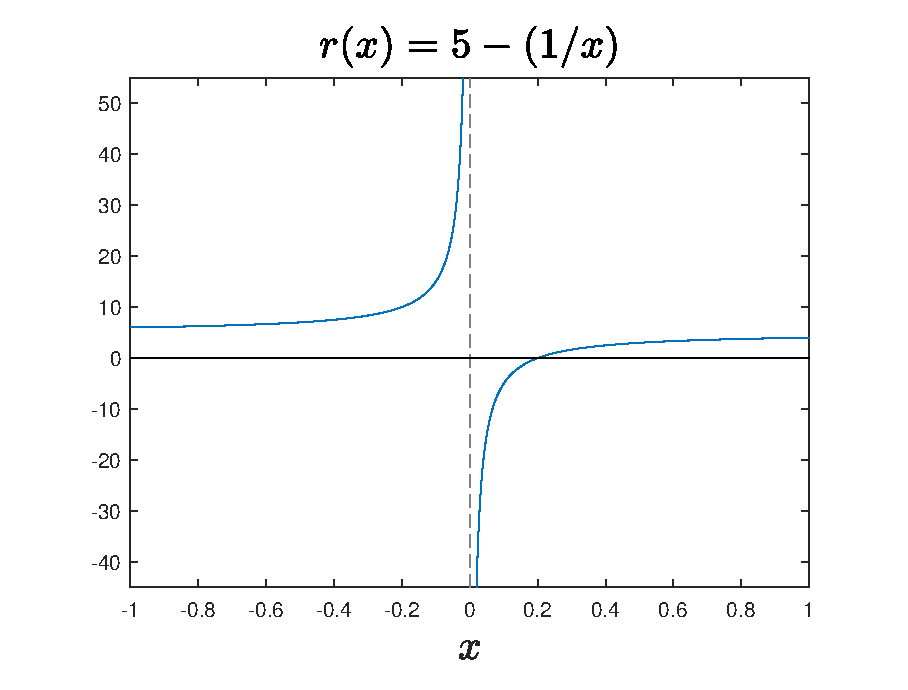
\includegraphics[width=.6\textwidth]{figs/recip_by_newton_function}
% \end{figure}
% \subsection{}
% Give the mathematical form of Newton's method. Simplify to a format that does not require any division.

% \subsection{}
% Set $a = 5$ and $x_0 = 0.1$. Compute the Newton iterates $x_1$ and $x_2$.

% \subsection{}
% For arbitrary $a>0$, argue that the Newton iterates will converge to $1/a$ for any initial $x_0$ in the interval $(0, 2/a)$. \emph{Hint:} First use the plot to argue for $0<x_0<1/a$.

% \subsection{}
% What happens when $x_0 = 2/a$? Does this contradict the local quadratic convergence of Newton's method?

\section{Newton's method and roots with higher multiplicity}
In the HW we have an example showing that Newton's method no longer converges quadratically if the root has higher than one multiplicity. We explore some more in this direction.

We first define multiplicity: $r\in \mathbb{R}$ is a root of multiplicity $m$ for the equation $f(x)=0$ if there is a function $h(x)$ such that $h(r)\neq 0$ and $f(x) = (x-r)^m h(x)$.

\subsection{}
Suppose that a function $f$ has $m$ continuous derivative on the interval $(a,b)$ containing $c$ (i.e. $f(x)\in C^m_{(a,b)}$). Show that $f$ has a zero of multiplicity $m$ at $c$ if and only if
\begin{align*}
    0 = f(r) = f'(r) = \dots = f^{(m-1)}(r)
\end{align*}
and
\begin{align*}
    f^{m}(r) \neq 0.
\end{align*}

\subsection{}
Suppose $r$ is a zero of multiplicity $m$ of $f$, and $f(x)\in C^m_{(a,b)}$, $r\in (a,b)$. Show that the following fixed-point method has $g'(r) = 0$:
\begin{align*}
    g(x) = x-m\frac{f(x)}{f'(x)}.
\end{align*}
What can you say about the convergence behavior of this fixed-point method?

\subsection{}
Code this modified Newton's method to solve $f(x) = x^2 = 0$. Check the convergence numerically. How do you plan to show this?

% \section{Bisection and Secant methods***}
% Define the cubic polynomial
% \[
% p(x) := (2x-1) (2x-3) (x-4).
% \]
% The following tasks can be done in any order.

% \subsection{}
% What are the three roots of $p$?

% \subsection{}
% Give numbers $a$ and $b$ such that the bisection method, when applied with
% initial interval $[a,b]$, is guaranteed to find the root $x^* = 3/2$ with enough iterations.

% \subsection{}
% From the initial points $x_0 = 0$ and $x_1 = 1.4$, 
% apply the secant method
% to compute $x_2$ and $x_3$. Can you guess the value of 
% \[
% \lim_{k \to \infty} x_k?
% \]
% How does this limiting value compare with the root you expect
% to find from the bisection method with initial interval $[0,1.4]$?

% \subsection{}
% The following table is a printout of the first 15 iterations of
% the secant method starting from $x_0 = 1.25$ and $x_1 = 3.9$.
% (Values are truncated to 4 significant digits.)

% \begin{table}[H]
% \centering
% \texttt{
% \begin{tabular}{|r|r|r|r|r|}
% \hline
% $k$ & $x_k$ & $f(x_k)$ & $x_k - 4$ & $|x_{k+1} - 4|/|x_k - 4|$ \\
% \hline
% 0 & +1.2500e+00 & +2.0625e+00 & -2.7500e+00 & +3.6363e-02 \\
% \hline
% 1 & +3.9000e+00 & -3.2640e+00 & -1.0000e-01 & +1.7238e+01 \\
% \hline
% 2 & +2.2761e+00 & -9.5053e+00 & -1.7238e+00 & +4.3461e-01 \\
% \hline
% 3 & +4.7492e+00 & +4.1377e+01 & +7.4923e-01 & +1.6842e+00 \\
% \hline
% 4 & +2.7381e+00 & -1.3986e+01 & -1.2618e+00 & +5.9736e-01 \\
% \hline
% 5 & +3.2461e+00 & -1.4459e+01 & -7.5381e-01 & +2.1637e+01 \\
% \hline
% 6 & -1.2310e+01 & -1.1542e+04 & -1.6310e+01 & +4.5020e-02 \\
% \hline
% 7 & +3.2657e+00 & -1.4343e+01 & -7.3429e-01 & +9.7360e-01 \\
% \hline
% 8 & +3.2850e+00 & -1.4217e+01 & -7.1491e-01 & +2.0501e+00 \\
% \hline
% 9 & +5.4656e+00 & +1.1544e+02 & +1.4656e+00 & +3.2465e-01 \\
% \hline
% 10 & +3.5241e+00 & -1.1651e+01 & -4.7582e-01 & +6.2596e-01 \\
% \hline
% 11 & +3.7021e+00 & -8.4013e+00 & -2.9785e-01 & +5.4478e-01 \\
% \hline
% 12 & +4.1622e+00 & +6.3283e+00 & +1.6226e-01 & +2.1825e-01 \\
% \hline
% 13 & +3.9645e+00 & -1.2096e+00 & -3.5415e-02 & +1.0428e-01 \\
% \hline
% 14 & +3.9963e+00 & -1.2894e-01 & -3.6934e-03 & +2.4787e-02 \\
% \hline
% 15 & +4.0000e+00 & +3.2045e-03 & +9.1551e-05 & +2.5374e-03 \\
% \hline
% 16 & +3.9999e+00 & -8.1306e-06 & -2.3230e-07 & N/A \\
% \hline
% \end{tabular}}
% \end{table}

% \begin{enumerate}
% \item Discuss what happens when computing $x_6$.
% \item At what rate does $x_k \to 4$? 
%     Justify your answer with observations from the table.
% \end{enumerate}
% -----------------------------------
% -----------------------------------
\chapter{Solving Linear Systems}
\section{Solving $Ax=b$ and LU factorization}
We will study the LU-factorization of the matrix
\begin{align*}
    A:=
  \begin{bmatrix}
    3  &   3   &    0\\
    6  &   4   &  7\\
    -6 &  -8   &   9
  \end{bmatrix}
\end{align*}
into the product
\begin{align*}
A = LU =
\begin{bmatrix}
1 & 0 & 0 \\
    \ell_{21} & 1 & 0\\
    \ell_{31} & \ell_{32} & 1
\end{bmatrix}
\begin{bmatrix}
    u_{11} & u_{12} & u_{13} \\
    0 & u_{22} & u_{23}\\
    0 & 0 & u_{33}
\end{bmatrix}
\end{align*}

\subsection{}
MATLAB matrices creation and array indexing.
\begin{enumerate}
    \item Create matrix $A$ in your favorite coding language.
    \item Print one element of the matrix via array indexing.
\end{enumerate}

\subsection{}
In practical Gaussian elimination, the matrices $L_k$, are never formed and multiplied explicitly. The multipliers $\ell_{jk}$ are computed and stored directly into $L$, and the transformations $L_k$ are then applied implicitly \cite[p.151]{TrefethenBau_97}.

\begin{enumerate}
    \item Verify that Gaussian elimination could be written as the following loop:
    \begin{figure}[H]
        \centering
        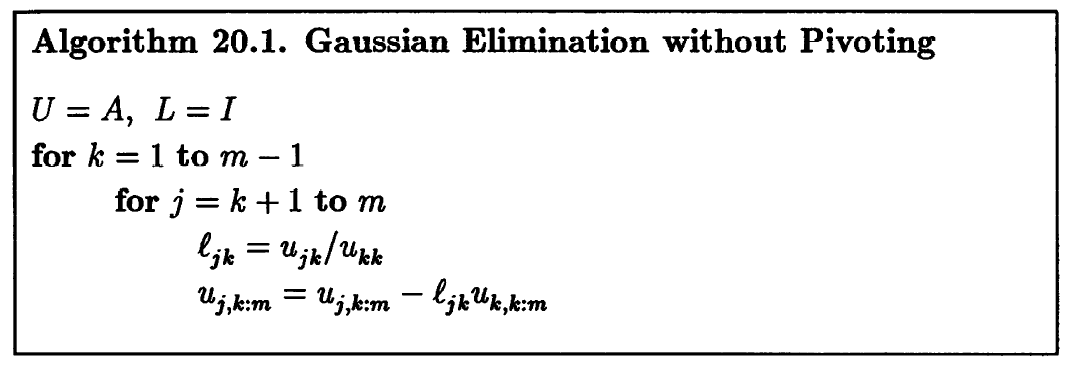
\includegraphics[width = 0.7\textwidth]{Session_2/latex/figs/TB97_Guass_wo_piv}
    \end{figure}
    \item Apply this loop at the matrix $A$ and obtain the $L$ and $U$ matrices.
\end{enumerate}

\subsection{}
Use the LU factorization to solve the linear system $Ax=b$ with
  $b=[1, 0, 0]^\top$ using one forward and one backward substitution.
  
\subsection{}\label{sec:3.1d}
Use the LU factorization to compute the determinant of
$A$. Recall that for two matrices of appropriate sizes,
$\det(AB)=\det(A)\det(B)$.
  
\subsection{***}
In the matrix $A$ defined above, replace the $(2,2)$-entry by $6$.
What is the rank of $A$ after this modification?
Attempt to compute the LU factorization of $A$. 
What do you observe?
How might you ``fix" the problem?

\section{Block matrices and MATLAB matrix operations}
\subsection{}
Let's practice creating matrices on the computer:
\begin{enumerate}
    \item Create a matrix of all ones in your favorite coding language.
    \item Create a matrix where its entries are independent standard Gaussian random variables (i.e.: with density $\mcal{N}(0,1)$). 
\end{enumerate}

\subsection{}
Now let's operate on these matrices:
\begin{enumerate}
    \item Sum two matrices.
    \item Multiply a matrix with an appropriately sized vector.
    \item Multiply two matrices (Try some non-square matrices).
\end{enumerate}

\subsection{}
Suppose we split up a matrix of size $\mathbb{R}^{(m+n)\times(m+n)}$ into blocks:
\begin{align*}
    A = \left[\begin{array}{c|c} A_{11} & A_{12} \\\hline A_{21} & A_{22} \end{array}\right]
\end{align*}
where $A_{11}\in\mathbb{R}^{n\times n}$, $A_{22}\in\mathbb{R}^{m\times m}$, $A_{12}\in\mathbb{R}^{n\times m}$, and $A_{21}\in\mathbb{R}^{m\times n}$. 

We have the block matrix multiplication formula:
\begin{align*}
    AB = \left[
\begin{array}{c|c} A_{11} & A_{12} \\\hline A_{21} & A_{22} \end{array} \right]\cdot
\left[
\begin{array}{c|c} B_{11} & B_{12} \\\hline B_{21} & B_{22} \end{array} \right]
= 
\left[
\begin{array}{c|c} A_{11}B_{11}+A_{12}B_{21} & A_{11}B_{12}+A_{12}B_{22} \\\hline A_{21}B_{11}+A_{22}B_{21} & A_{21}B_{12}+A_{22}B_{22} \end{array} \right]
\end{align*}

You could try to prove this at home. In session, we will verify this formula numerically by creating examples of $A$ and $B$.

\begin{enumerate}
    \item Make $A$ and $B$ to be Gaussian random matrices.
    \item How do you compare two matrices numerically?
\end{enumerate}

\subsection{}
(Challenge for you) Could you calculate the determinant of $A\in \mathbb{R}^{(m+n)\times(m+n)}$ by calculating the determinants of only $m$-by-$m$ and $n$-by-$n$ matrices? 

Hint: try Gaussian elimination on block matrices. Then follow the procedure in \ref{sec:3.1d}.

\section{Schur complement}
Assume $M\in \mathbb{R}^{(m+n)\times(m+n)}$ and we split them into blocks
\begin{align*}
    M = \begin{bmatrix}
    A &B\\
    C &D
    \end{bmatrix}
\end{align*}
where $A\in\mathbb{R}^{n\times n}$, $D\in\mathbb{R}^{m\times m}$, $B\in\mathbb{R}^{n\times m}$, and $C\in\mathbb{R}^{m\times n}$. We also assume that $M$ and all its leading submatrices are non-singular. 

\subsection{}
Verify the formula
\begin{align*}
     \begin{bmatrix}
    I & \\
    -CA^{-1} & I
    \end{bmatrix} \begin{bmatrix}
    A &B\\
    C &D
    \end{bmatrix} =  \begin{bmatrix}
    A &B\\
     &D-CA^{-1}B
    \end{bmatrix}
\end{align*}
for ``elimination" of the block $C$. The matrix $D-CA^{-1}B$ is  known as the \textit{Schur complement} of $A$ in $M$.

\subsection{}
Explain the above decomposition as a form of ``block LU''. 

Extra: Write down the block LDU decomposition. 

\section{Diagonally dominant matrix and pivoting}
A matrix is called strictly (column) diagonal-dominant if the
 the absolute value of the diagonal entry in each column is larger than
 the sum of the absolute values of the other entries in that
 column; i.e., for all $i$:
 $$
 |a_{ii}|>\sum_{j=1, j\not=i}^n |a_{ji}|
 $$
 
\subsection{}
Which of the following matrices is diagonally dominant?
$$
 B={\begin{bmatrix}-2&2&1\\1&3&2\\1&-2&0\end{bmatrix}}, \qquad
 C={\begin{bmatrix}-4&2&1\\1&6&2\\1&-2&5\end{bmatrix}}
$$

\subsection{}
When computing the LU
 factorization of a strictly diagonally dominant matrix, why is
 pivoting never necessary? 

\begin{enumerate}
    \item First argue why the first column does not require pivoting. Then use Gaussian elimination to generate the required zeros in the first column
    \item Show that, the submatrix you obtain when removing the first column and row is again strictly  diagonally dominant.
\end{enumerate}

\subsection{}
Let's show that an LU decomposition without pivoting exists in a different way:
  \begin{enumerate}
    \item Why are the leading principal submatrices of a strictly
      diagonally dominant matrix also strictly diagonally dominant?
    \item Show that a diagonally dominant matrix is always invertible
      using the following argument: If $A$ is not invertible, then
      there must exists a vector $\vec v\not=0$ such that
      $A\vec v = \vec 0$. Call $r$ the largest (in
      absolute value) entry of $\vec v$ and consider
      multiplication of the $r$-th row. 
    \item Combine the previous two statements with a result from class
      to argue that the LU factorization of a strictly diagonally
      dominant matrix exists.
 \end{enumerate}
 
\begin{figure}[H]
    \centering
    
\includegraphics[scale = 0.7]{Session_3/latex/figs/pivot_pivot}
\end{figure}



\section{Calculating pivoted-LU}
Compute by hand an LU factorization with pivoting ($PA = LU$) of the matrix:
\begin{align*}
A:=
  \begin{bmatrix}
    -2  &   0   &   6\\
    -3  &   6   &   9\\
    -1 &    4   &   5
  \end{bmatrix}.
\end{align*}
Double-check your result using MATLAB's or Python's LU function!
% -----------------------------------
% -----------------------------------
\chapter{Conditioning and Stability}
\section{Matrix norms basics}
\subsection{}
Compute $\|A\|_\infty$ and $\|A\|_1$ for the matrix
\[
A = \begin{bmatrix}
1 & -1  &2 & -3 \\ 7 & 2 & 3 & 5 \\ 2 & -4 & 3 & 8 \\ -3 & 5 & 3 & 1
\end{bmatrix}.
\]

% \subsection{}
% Find $\|{A}\|_2$ for the matrix 
% \[
% A = \begin{bmatrix} 1 & \varepsilon \\ \varepsilon & 1 \end{bmatrix},
% \]where $\varepsilon \in (0,1)$ (Hint: for symmetric matrices $A$, the
% eigenvalues of $A^T A$ are simply the squares of the eigenvalues of
% $A$).

\subsection{}
Show that for symmetric positive definite (i.e., all eigenvalues
  are positive) matrices $A\in \mathbb R^{n\times n}$, the 2-norm
  condition number can also be computed as the ratio between the
  largest and the smallest eigenvalue of $A$, i.e.:
  $\kappa_2(A)=\lambda_{\max}/\lambda_{\min}$. Hint: Think about what
  the largest eigenvalue of $A^{-1}$ is.

\section{Norms Equivalency}
Two norms in a finite-dimensional linear space $X$ (e.g.: $\mathbb{R}^n$), $\norm{\;\cdot\;}_a$ and $\norm{\;\cdot\;}_b$, are called equivalent if there is a constant $c$ such that for all $x$ in $X$,
\begin{align}
    \norm{x}_a\leq c\norm{x}_b,\qquad \norm{x}_b\leq c\norm{x}_a.\label{eq:norm_equiv}
\end{align}

\subsection{}
Suppose $\norm{\;\cdot\;}_a$ and $\norm{\;\cdot\;}_b$ are equivalent, and we know that an algorithm produces a sequence of vectors $\{e_n\}_{n\geq 1}$, $\norm{e_n}_a\to 0$ as $n\to\infty$. What could we conclude about $\norm{e_n}_b$'s behavior for $n\to\infty$?

\subsection{}
We first show that the vector norms on $\mathbb{R}^n$, $\norm{\;\cdot\;}_{2}$ and $\norm{\;\cdot\;}_{\infty}$, are equivalent. To do this prove the inequality:
\begin{align*}
    \norm{x}_\infty \leq \norm{x}_2 \leq \sqrt{n}\norm{x}_\infty.
\end{align*}

\subsection{}
The induced matrix norm on $\mathbb{R}^{n\times n}$: $\norm{\;\cdot\;}_{2}$ and $\norm{\;\cdot\;}_{\infty}$ are equivalent as well. Prove the inequality
\begin{align*}
    &\norm{A}_\infty \leq \sqrt{n}\norm{A}_2,\\
    &\norm{A}_2 \leq \sqrt{n}\norm{A}_\infty.
\end{align*}

\subsection{}
(Challenge) Prove that: in a finite-dimensional linear space, all norms are equivalent; that is, any two satisfy \eqref{eq:norm_equiv} with some $c$, depending on the pair of norms \cite[p.217]{Lax_07}.

One inequality is relatively simple, the other one requires some big theorems from analysis. Read about the proof in Lax's book if you are interested.

\section{Condition numbers based on different norms}
\subsection{}
Let $A \in \mathbb{R}^{n\times n}$ be defined by
\begin{equation*}
    A = %
    \begin{bmatrix}
      1      & 0      & 0      & 0      &  0      \\ 
      1      & 1      & 0      & 0      &  0      \\
      1      & 0      & 1      & 0      &  0      \\
      \vdots & \vdots & \vdots & \ddots &  \vdots \\
      1      & 0      & 0      & 0      &  1
    \end{bmatrix}.
\end{equation*}
Calculate $\kappa_1(A)$ and $\kappa_\infty(A)$. We see that a matrix can be well or ill-conditioned depending on the choice of norms.

\subsection{}
Indeed, we solve $A\ve x = \ve b$ and $A(\ve x+\Delta \ve x) = (\ve b+\Delta \ve b)$ where
\begin{align*}
    \ve b = \begin{bmatrix}
    1\\1\\\vdots\\1
    \end{bmatrix},\qquad \ve x = \begin{bmatrix}
    1\\0\\\vdots\\0
    \end{bmatrix},\qdt{and} \Delta\ve b = \begin{bmatrix}
    \epsilon\\0\\\vdots\\0
    \end{bmatrix}
\end{align*}
Check that we have for both norms:
\begin{align*}
    \frac{\norm{\Delta\ve x}}{\norm{\ve x}} \leq \kappa(A)\frac{\norm{\Delta\ve b}}{\norm{\ve b}}.
\end{align*}

\section{Conditional number for the Hilbert matrix***}  
The Hilbert matrix $H\in \mathbb R^{n\times n}$ is a matrix with
  entries
  $$
  h_{ij} = \frac{1}{i+j-1}.
  $$ 
\subsection{}
Using MATLAB or Python, compute the 2-norm-based condition
  numbers for $n=3,5,10,20,25$.  
  
\subsection{}
  Let's consider a relative right hand
  side perturbation $\delta\boldsymbol b$ of a linear system with
  $\|\delta\boldsymbol b\|_2/\|\boldsymbol b\|_2\approx
  10^{-15}$. Write down the corresponding bounds $\|\delta\boldsymbol
  x\|_2/\|\boldsymbol x\|_2$ from the theory we discussed in class.

\subsection{}
  Now, let's compute the actual error. Use the right-hand side vector
  with entries $b_i = \sum_{j=1}^n(j/(i+j-1))$ chosen such that the
  solution vector has entries $x_i=i$. Now, Compute the numerical
  solutions\footnote{Note that all these computations contain tiny
    errors due to the final precision of computer computations.}
  $\boldsymbol x$, then re-compute $\boldsymbol b=H\boldsymbol x$ and
  compare the relative right-hand side error and the relative error
  in the solutions. How much are these better than the estimates you
  got from the condition number?
  
\section{Condition numbers and pivoted LU}
\subsection{}
Solve the matrix equation $A\boldsymbol x = \boldsymbol b$ with 
\begin{align*}
  A:=
  \begin{bmatrix}
    1       & 0  \\
    10^{4}  & 1
  \end{bmatrix}
  \qdt{ and }
  \boldsymbol b = \begin{bmatrix}
  0\\1
  \end{bmatrix}.
\end{align*}
What is $\kappa_\infty(A)$?

Consider a small perturbation $\Delta \boldsymbol b=[10^{-3},0]^\top$ being added to the right-hand side, and solve again. Repeat with $\Delta \boldsymbol b =[0,10^{-3}]^\top$. You should see that small perturbation can, but does not have to have a large effect even for badly conditioned systems.

\subsection{}
Verify the following LU decomposition of a matrix $A$ without pivoting:
  $$
  A := \begin{bmatrix} 10^{-4} & 1\\ 1 & 1
  \end{bmatrix} = LU =
  \begin{bmatrix} 1 & 0\\ 10^4 & 1
  \end{bmatrix}
  \begin{bmatrix} 10^{-4} & 1\\ 0 & 1-10^4
  \end{bmatrix}
  $$ 
We have seen in the previous problem that solving a system with the matrix $L$ is sensitive to errors, i.e., it is poorly conditioned. However, the original $A$ matrix is well-conditioned.

Now the LU factorization of $A$ with pivoting is
\begin{align*}
PA = \begin{bmatrix} 1 & 1 \\ 10^{-4} & 1
  \end{bmatrix} = LU =
  \begin{bmatrix} 1 & 0\\ 10^{-4} & 1
  \end{bmatrix}
  \begin{bmatrix} 1 & 1\\ 0 & 1-10^{-4}
  \end{bmatrix}
\end{align*}
We see that the LU factors with pivoting are better conditioned.

\section{Condition number for solving linear system}  
\subsection{}
Find $\|{A}\|_2$ for the matrix 
\[
A = \begin{bmatrix} 1 & \varepsilon \\ \varepsilon & 1 \end{bmatrix},
\]where $\varepsilon \in (0,1)$ (Hint: for symmetric matrices $A$, the
eigenvalues of $A^T A$ are simply the squares of the eigenvalues of
$A$).

\subsection{}
Continued from the previous item: Suppose that you have two systems
\begin{align*}
\begin{matrix}
x_1 + \varepsilon x_2 = b_1 \\
 \varepsilon x_1 + x_2 = b_2  
\end{matrix}\qquad \text{and}\qquad
\begin{matrix}
\tilde x_1 + \varepsilon \tilde x_2 = \tilde b_1 \\
 \varepsilon \tilde x_1 + \tilde x_2 = \tilde b_2
\end{matrix}
\end{align*}
where $\tilde{\boldsymbol b} = (\tilde b_1, \tilde b_2)^T$ is
approximately equal to ${\boldsymbol b}=( b_1, b_2)^T$, with a $5\%$
relative error, that is $\frac{\|{\tilde {\boldsymbol b} -
    {\boldsymbol b}}\|_2}{\|{{\boldsymbol b}}\|_2} \leq 0.05$.  Find
an upper bound for the relative error $\frac{\|\tilde {\boldsymbol x}
  - {\boldsymbol x}\|_2}{\|{\boldsymbol x}\|_2}$ where $\tilde
{\boldsymbol x} = (\tilde x_1, \tilde x_2)^T$ and ${\boldsymbol x} =
(x_1,x_2)^T$. This upper bound will depend on $\varepsilon$.
% -----------------------------------
% -----------------------------------
\chapter{QR Factorization and Least Squares}
\section{Two forms of QR}
\subsection{}
We have two forms of QR:
\begin{figure}[H]
    \centering
    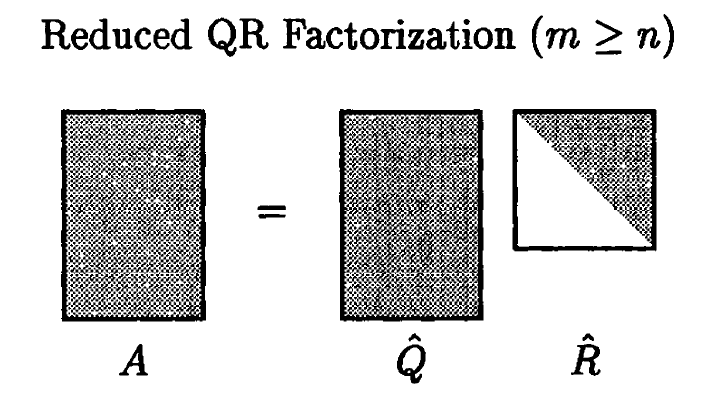
\includegraphics[width = 0.45\textwidth]{Session_5/latex/figs/TB_reducedQR}
    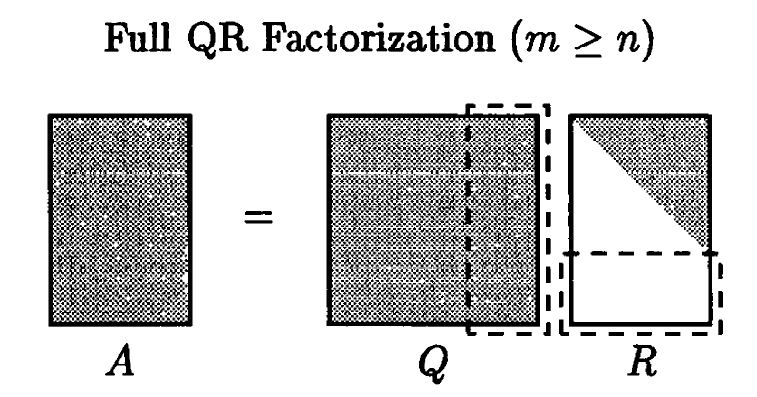
\includegraphics[width = 0.45\textwidth]{Session_5/latex/figs/TB_fullQR}
\end{figure}

\subsection{}
We can interpret the formula for the solution of the least-squares problem
\begin{align*}
    \hat R \ve x = \hat Q^\top \ve b
\end{align*}
by using the full form of QR.

\section{Projectors}
A projector is a square matrix $P$ that satisfies
\begin{align*}
    P^2 = P.
\end{align*}

\subsection{}
Assume $P$ is a projector, and show that $I-P$ is also a projector.

\subsection{}
We can show that
\begin{align*}
    & \text{range}(I-P) = \text{null}(P);\\
    & \text{null}(I-P) = \text{range}(P);\\
    & \text{range}(P) \cap \text{null}(P) = 0.
\end{align*}

An orthogonal projector is a projector whose has the subspaces $\text{range}(P)$ and $\text{null}(P)$ orthogonal.

n.b.: An orthogonal projector $P$ is not an orthogonal matrix! Why?

\subsection{}
Show that if $P=P^\top$ symmetric, the projector $P$ is orthogonal (Hint: take one vector in $\text{range}(P)$ and one in $\text{null}(P)$, show that they must be orthogonal to each other). 

The reverse direction holds as well. Therefore the two definitions are equivalent.

\subsection{}
A special case of orthogonal projection is the projection onto a vector:
\begin{align*}
    P_v = \frac{\ve v \ve v^\top}{\ve v^\top \ve v}.
\end{align*}
Show that it is indeed an orthogonal projector with range $\text{span}(\ve v)$.

\subsection{}
Another orthogonal projection is
\begin{align*}
    P_{\perp v} = I-\frac{\ve v \ve v^\top}{\ve v^\top \ve v}.
\end{align*}
What is its null space? What is its range?

\section{Geometric interpretation of Householder reflectors}
\subsection{}
Name $H(\ve v)$ the linear subspace orthogonal to the vector $\ve v$. A reflector across $H(\ve v)$ is 
\begin{align*}
    F_{\ve v} = I - 2 \frac{\ve v \ve v^\top}{\ve v^\top \ve v}.
\end{align*}
Compare this with $P_v$ and $P_{\perp v}$, and interpret the formula geometrically.

\begin{figure}[H]
    \centering
    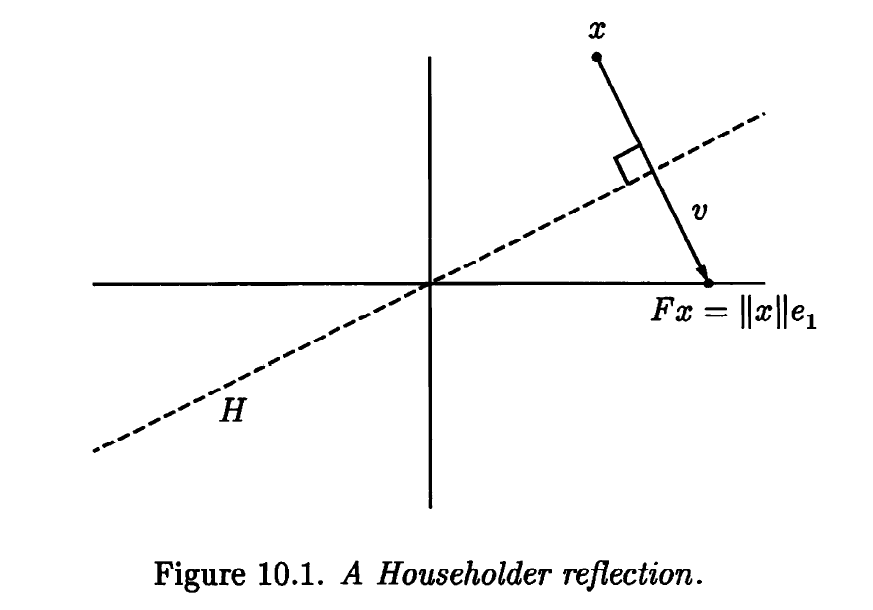
\includegraphics[width = 0.6\textwidth]{Session_7/latex/figs/TB_HouseholderRef}
\end{figure}

\subsection{}
To use Householder for QR decomposition, we want $F\ve x = c\ve e_1$. We know that $c = \pm\norm{\ve x}_2$. Explain this geometrically.

\subsection{}
From this, we have that
\begin{align*}
    \ve v = \ve x- F\ve x =  \ve x \pm \norm{\ve x}\ve e_1.
\end{align*}
From a geometric point of view, why is this the correct formula?

\section{QR decomposition via Householder}
\subsection{}
Construct the QR factorization of the following matrix
  using Householder reflectors (the algebra is not simple. You might use MATLAB as a calculator):
\begin{align*}
{A} = 
\begin{bmatrix}
1 & 0 & 1 \\
2 & 1 & 3 \\
0 & 2 & 4
\end{bmatrix}.
\end{align*}
\subsection{}
Use the factorization to determine $|\det(A)|$

\section{Least squares and infections disease}
Let us assume an infectious disease with the following reported new
infections $I_i$ on each day $t_i$, for $i=1,\ldots,10$.
\begin{table}[h]\centering
  \caption{Number of new infections $I_i$ on days $t_i$.}
  \begin{tabular}{c||c|c|c|c|c|c|c|c|c|c|}
\hline
$t_i$: & 1 & 2 & 3 & 4 & 5 & 6 & 7 & 8 & 9 & 10\\ \hline
$I_i$: & 14 & 20 & 21 & 24 & 15 & 45 & 67 & 150 & 422 & 987\\ \hline
\end{tabular}
\end{table}
Using least squares fitting, we would like to understand the nature of
this growth. We consider two models to describe the connection between
time (i.e., days) $t$ and the number of new infections, both with 3
unknown parameters $(a,b,c)$:
\begin{equation*}%\label{poly}
  I(t) = a + b t + c t^2 \qquad \text{(polynomial model)}
\end{equation*}
\begin{equation*}%\label{exp}
  I(t) = a + bt + c\exp(t) \qquad \text{(exponential model)}
\end{equation*}
Our goal is to figure out which model describes the progression of the
infections better, and we use least squares fitting to figure that
out. Note that if a model would fit the data perfectly, $I(t_i) = I_i$
for all $i$. In general, you will not be able to find parameters that
satisfy this, and thus have to use least squares fitting (sometimes
this is also called \emph{regression}).

\subsection{} Formulate, assuming the polynomial model, the least squares
  problem for the parameters $\boldsymbol x=[a,b,c]^T$ by specifying the
  matrices $A$ and the vector $\boldsymbol b$:
  $$ \min_{\boldsymbol x\in \mathbb R^3}\|A\boldsymbol x - \boldsymbol
  b \|_2^2
  $$

\subsection{}  Same as above, but for the exponential model.

\subsection{} Use a QR-factorization in MATLAB or Python to solve these
  problems and plot the data as points, as well as the model as a
  line. Repeat using the normal equations $A^TA\boldsymbol x =
  A^T\boldsymbol b$.
\subsection{} To decide which model describes the data better, we need to
  compute the distance between the model and the data points. Take a
  look at the proof from class for how  the QR  factorization can be
  used to solve least squares  problems. In  particular, we found
  that:
  $$
  \|A\boldsymbol x  - \boldsymbol  b\|_2^2 \ge \|\boldsymbol b_2\|_2^2,
  $$ where $\boldsymbol b_2 = \hat{\hat Q}^\top\boldsymbol b$. We also
  found that this inequality is equality if $\boldsymbol x$ solves
  the least squares problem. Thus, the norm or $\boldsymbol b_2$ is a
  measure of how well the model fits the data. Use this to decide
  which of the two models above describes the data better.
% -----------------------------------
% -----------------------------------
\chapter{Eigen-Problems}
\section{Gershgorin disks and the power method}
Consider the matrix 
$$
A = \begin{bmatrix}
- 6 & 2 & 0.3 & 0 & -0.7 \\
2 & - 4 & 0.1 & 0.05 & 0 \\
0.3 & 0.1 & 2 & 0.1 & 0.1 \\
0 & 0.05 & 0.1 &  4 & 0 \\
-0.7 & 0 & 0.1  & 0  & 6
\end{bmatrix}
$$
and recall the definition of the Gershgorin disks:
\[
D_i = \{ z \in \mathbb C ~|~ |z - a_{ii}| \le \sum_{j \ne i} |a_{ij}| \}.
\]

\subsection{}
Argue that all eigenvalues of $A$ are real.

\subsection{}
What are the Gershgorin disks for $A$?  Use them to give a set, $D \subset \mathbb{R}$, that contains all eigenvalues of $A$.

\subsection{}
Can you conclude that the eigenvalue with the largest absolute value is simple?

\subsection{}
Argue that $A$ is invertible. Conclude that all diagonally dominant matrix is invertible.

\subsection{}
True or False? Let $A \in \mathbb{R}^{n \times n}$ and $D_i$, $i
  = 1,2,\dots,n$, be the Gerschgorin disks of $A$. If $0 \in
  \bigcup_{i=1}^n D_i$ then $A$ is singular.
  
\subsection{}
Write down the first iteration of the power method starting from $\ve x_0 = (0,0,0,0,1)^T$.
You don't need to normalize.
Explain why $\ve x_0 = \ve 0$ is not a suitable starting point.

\subsection{}
The eigenvalues of $A$, after rounding, are $\{-7, -3, 2, 4, 6\}$.
Which eigenvalue direction will the sequence of the previous question converge to?

\section{Eigenvectors as stationary points of Rayleigh quotient}
% Let $H$ be a real symmetric matrix. Denote the eigenvalues of $H$, arranged in increasing order, by $a_1,\dots,a_n$. Then we have that
% \begin{align*}
%     a_j = \min_{\dim S = j}\max_{x\in S,x\neq 0} \frac{x^\top Hx}{x^\top x}
% \end{align*}
% where $S$ is a linear subspace of $X$ \cite[p.116]{Lax_07}.

For $H$ a real symmetric matrix, we define Rayleigh quotient as a function $\mathbb{R}^n\to\mathbb{R}$:
\begin{align*}
    R(\ve x) = \frac{\ve x^\top H\ve x}{\ve x^\top \ve x} = \frac{q(\ve x)}{p(\ve x)}.
\end{align*}
We will show that $\ve v$ is a stationary point (i.e.: $\nabla R(\ve v) = 0$) of the Rayleigh quotient if and only if it is an eigenvector of $H$ (cf. \cite[p.114-116]{Lax_07} and \cite[p.203-204]{TrefethenBau_97}).

\subsection{}
To characterize a point such that $\nabla R(\ve v) = 0$, we need to know the gradient of $R(\ve x)$ at $\ve v$. We could do this, but an alternative approach is to take $t\in \mathbb{R}$ and calculate
\begin{align*}
    \left.\frac{\de}{\de t} R(\ve v+t\ve y)\right|_{t=0}
\end{align*}
for all $\ve y\in\mathbb{R}^n$. In particular, we can get the gradient by picking $\ve y = \ve e_i$.

\subsection{}
Using the above calculation, show the iff claim in the main text of the problem.

\section{Computing eigenvalues via the Power Iteration}
Given is the following matrix:
\[
A=\begin{bmatrix}
-2 & 1 & 4  \\ 1 & 1 & 1 \\ 4 & 1 & -2 \end{bmatrix},
\]
It has eigenvalues and eigenvectors:
\[
\lambda_1=0,
\, {\boldsymbol v_1}
=\begin{bmatrix}
0.41  \\ -0.82 \\ 0.41 \end{bmatrix},\quad
\lambda_2=-6,
\,{\boldsymbol v_2}
=\begin{bmatrix}
0.71  \\ 0.0 \\ -0.71 \end{bmatrix},\quad
\lambda_3=3, \,{\boldsymbol v_3}
=\begin{bmatrix}
-0.58  \\ -0.58 \\ -0.58 \end{bmatrix}.
\]

\subsection{}\label{sec:1.a}
Calculate the first iterate of the power method when ${\boldsymbol x_0}=(0,1,1)^T$.

\subsection{}
Which eigenvalue direction will the sequence defined in \ref{sec:1.a} converge to?
  
\subsection{}
Give an initialization vector such that the power method does \emph{not} converge to the direction of the largest (in absolute value) eigenvalue.
  
\subsection{}\label{sec:1d}
Write a simple program implementing the power method for the matrix $A$.
\begin{enumerate}
    \item Use the Rayleigh quotient to calculate estimates of the eigenvalues for each iteration.
    \item What is the order of convergence of the eigenvector estimates and the eigenvalue estimates? What is the speed of convergence?
    \item Could you explain the relationship between the two convergence speeds? \\
    (Hint: last week we showed that eigenvectors $\ve v$ are stationary points of the Rayleigh quotient)
\end{enumerate}

\section{The Inverse Iteration}
Take $A$ to be the matrix above, and let $\theta\in\mathbb{R}$ and let ${\boldsymbol x_0}\in\mathbb{R}^3$.
\subsection{}
Define the \emph{Inverse Iteration} (also called
  \emph{Inverse Power Method}) to calculate eigenvectors of $A$ near
  $\theta$.

\subsection{}
If $\theta=2$, where will the sequence defined in (i)
  converge to and why?

\subsection{}
If $\theta=-2$, where will the sequence defined in (i)
  converge to and why?

\subsection{}
Write a simple program implementing the inverse power method. Do the same sub-tasks as the ones in \ref{sec:1d}.

\section{The Rayleigh Quotient Iteration}
It is irresistible to use the eigenvalues estimates from the Rayleigh quotient to update $\theta$ for each step in the inverse iteration. The resulting algorithm is the Rayleigh Quotient Iteration \cite{TrefethenBau_97}:
\begin{figure}[H]
    \centering
    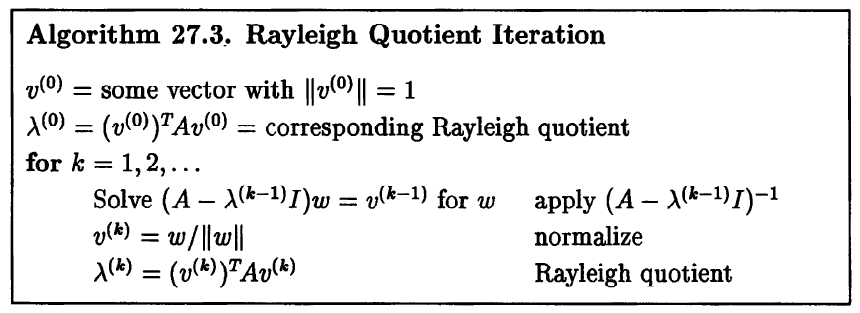
\includegraphics[width = 0.8\textwidth]{Session_9/latex/figs/TB_Rayleigh_Quo_Iter}
\end{figure}

\subsection{}
Implement the Rayleigh Quotient Iteration. 
\begin{enumerate}
    \item What is the order of convergence of the eigenvector estimates and the eigenvalue estimates?
    \item Could you explain this (high) order of convergence?
\end{enumerate}

\section{Singular Value Decomposition (SVD) basics}
\subsection{}
Like QR, SVD has the full and reduced form \cite{TrefethenBau_97}:
\begin{figure}[H]
    \centering
    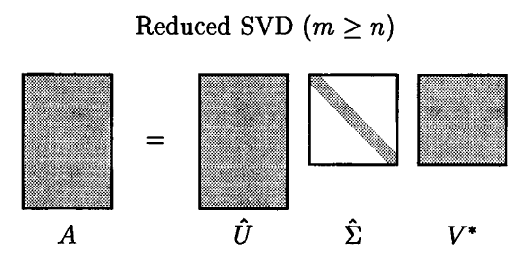
\includegraphics[width = 0.49\textwidth]{Session_10/latex/figs/TB_reducedSVD}
    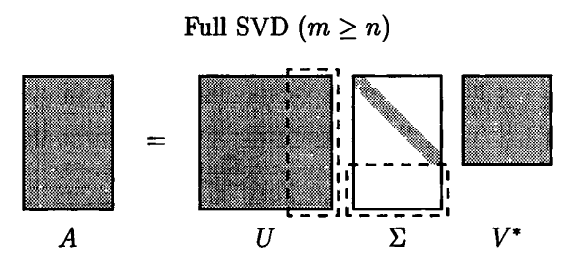
\includegraphics[width = 0.49\textwidth]{Session_10/latex/figs/TB_fullSVD}
\end{figure}
Note that the full form has $U$ which spans the whole of $\mathbb{R}^n$.

\subsection{}
We can interpret the full form of SVD as a change of basis, then a scaling, and then another change of basis (Figure from \cite{Strang_93}).
\begin{figure}[H]
    \centering
    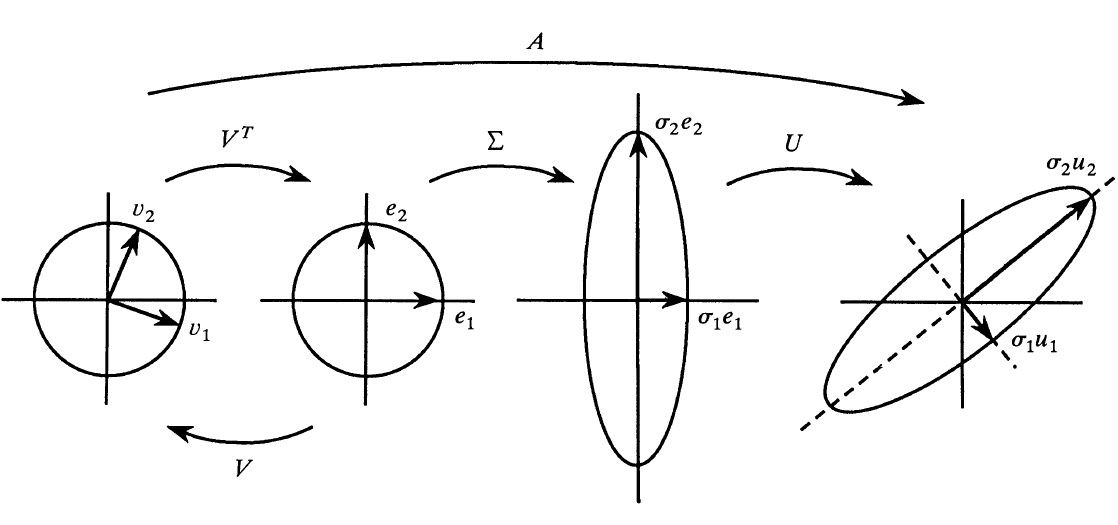
\includegraphics[width = 0.7\textwidth]{Session_10/latex/figs/strang_SVD}
\end{figure}

\section{Some properties of SVD}
We list (and attempt to prove) some properties of SVD:

\subsection{}
$\text{range}(A) = \text{span}(\ve u_1,\ve u_2,\dots,\ve u_r)$ and $\text{null}(A) = \text{span}(\ve v_{r+1},\dots,\ve v_n)$. 

\subsection{}
The rank of $A$ is $r$, the number of nonzero singular values.

\subsection{}
We have $\norm{A}_2 = \sigma_1$, the largest singular value. And $\norm{A}_F = \sqrt{\sigma_1^2+\sigma_2^2+\dots+\sigma_r^2}$. 

You will show the second property in your homework.

\section{Low-rang approximation using SVD}
\subsection{}
Show that $A$ is the sum of $r$ \emph{rank-one} matrices:
\begin{align*}
    A = \sum_{j=1}^r \sigma_j \ve u_j \ve v_j^\top.
\end{align*}

\subsection{}
For any $\nu$ with $0\leq \nu \leq r$, define
\begin{align*}
    A_\nu = \sum_{j=1}^\nu \sigma_j \ve u_j \ve v_j^\top.
\end{align*}
Then we have
\begin{align*}
    \norm{A-A_\nu}_2 = \inf_{\substack{B\in\mathbb{R}^{m\times n}\\\text{rank}(B)\leq\nu}}\norm{A-B}_2 = \sigma_{\nu+1}.
\end{align*}

Note that a similar theorem is also true for the Frobenius norm.
% -----------------------------------
% -----------------------------------
\chapter{Interpolations}
\section{Polynomial interpolation and linear algebra}
In lecture you have learned the theorem which states:

For $n\geq 1$ and distinct $n+1$ data pairs $(x_0,y_0),\dots,(x_n,y_n)$ there exists a unique $p_n(x)\in P_n$, an $n$-th order polynomial such that $p_n(x_i) = y_i$ for $i = 0,\dots,n$. 

We will try to prove this using linear algebra.

\subsection{}
We can write an $n$-th order polynomial as
\begin{align*}
    p_n(x) = a_0 + a_1x + \dots + a_nx^n.
\end{align*}
This gives us $n+1$ free variables to solve. Frame the problem of finding $p_n(x)$ s.t. $p_n(x_i) = y_i$ for $i = 0,\dots,n$ as a matrix problem $X\ve a = \ve y$.

\subsection{}
Show that since $x_i\neq x_j$ for all $i,j$, we have the matrix $X$ we constructed has full rank. 

\subsection{}
Think about the uniqueness and existence claim in the theorem in linear algebra language. 


\newpage
\bibliographystyle{alpha}
\bibliography{citation}

\end{document}